  

%%%%%%%%%%%%%%Empieza la presentacion%%%%%%%%%%%%%%%%%%%%%%%%%%%%%%%%%%%%

%\begin{frame}
%\frametitle{Esquema}
 %   \tableofcontents
%\end{frame}



\subsection{Caracterización en frecuencia de señales reales}

\begin{frame}
\frametitle{Caracterización en frecuencia de señales reales I}

\vspace{-0.2cm}

\footnotesize

\begin{itemize}

\item Las señales reales no suelen tener un comportamiento estacionario en frecuencia a lo largo del tiempo. Es decir, durante diferentes etapas (trozos temporales) de la señales habitual que aparezcan diferentes componentes en frecuencia.

\visible<2->{

\item Las Transformadas de Fourier que hemos visto hasta ahora (CTFT, DTFT, DFT) se aplican habitualmente sobre la señal completa, y por lo tanto, no nos permiten observar el cambio del comportamiento en frecuencia de una señal real a lo largo del tiempo. 
}

\visible<3->{

\item Para poder observar el cambio del comportamiento en frecuencia de la señal a lo largo del tiempo es necesario realizar las transformadas sobre diferentes trozos de la señal.

\vspace{-0.4cm}

\begin{columns}[c]
\begin{column}{6cm}

\lstinputlisting{./Matlab/Spect1Corte.m}

\end{column}

\hspace{-1cm}\begin{column}{4cm}
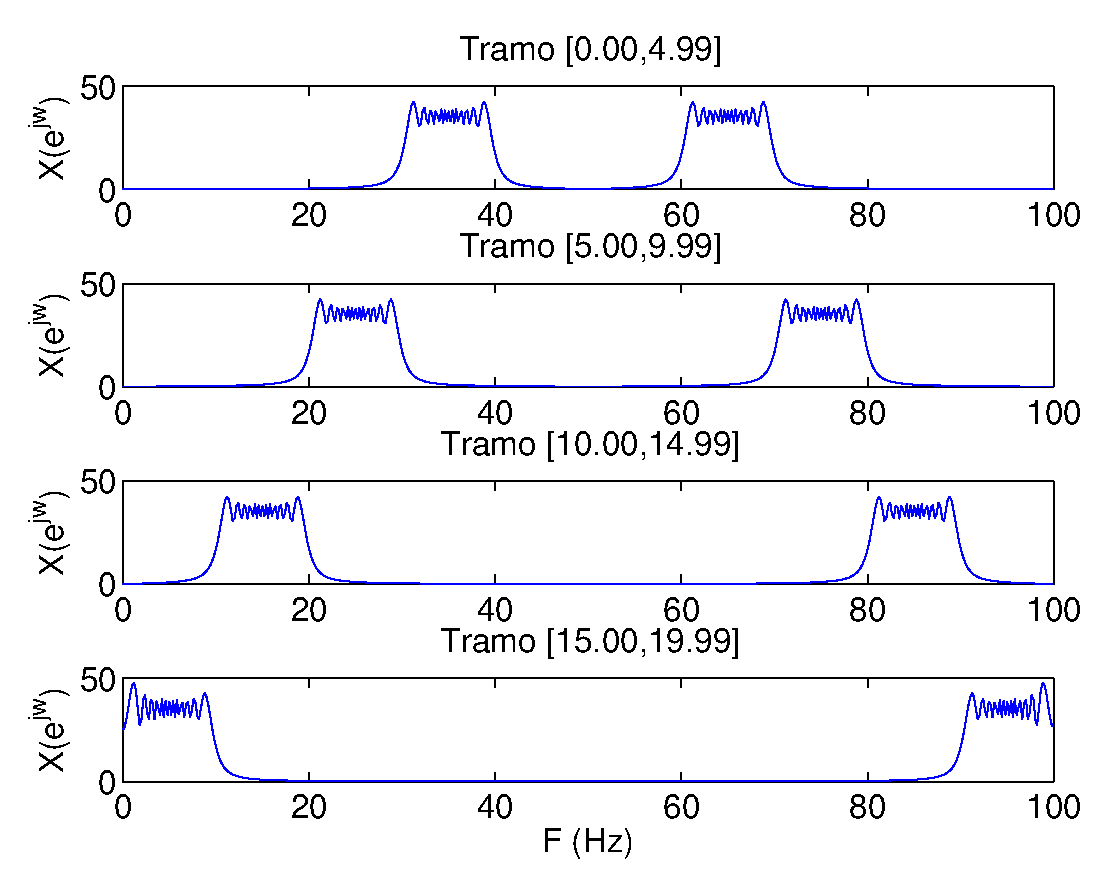
\includegraphics[width=4cm]{./Figures/Spect1.eps} 
\end{column}

\end{columns}
}

\end{itemize}

\end{frame}


%%%%%%%%%%%%%%%%

\begin{frame}
\frametitle{Caracterización en frecuencia de señales reales II}

\vspace{-0.2cm}

\scriptsize

\begin{itemize}



\item El truncamiento de la señal en trozos es equivalente a multiplicar la señal por una ventana rectangular.  El producto de una señal por una ventana rectangular hace que el espectro de la señal truncada sea la \alert{convolución} de las componentes en frecuencia del trozo de la señal elegido con el espectro en frecuencia del pulso rectangular del tamaño de la ventana. Esto provoca los rizos que se observan en la transformada de cada tramo.

\visible<2->{

\item Para evitar el fenómeno de Gibbs (rizos) propios de la ventana rectangular, se puede sustituir la ventana rectangular por cualquiera de las ventanas previamente estudiadas (triangular, hamming, etc)
}

\vspace{-0.3cm}

\begin{columns}[c]
\begin{column}{6cm}

\visible<3->{

\lstinputlisting{./Matlab/Spect2Corte.m}}

\end{column}

\hspace{-0.8cm}\begin{column}{4cm}

\scriptsize


\visible<4->{
\rotatebox{90}{\hspace{0.1cm}\textit{Ventana rectangular}}}
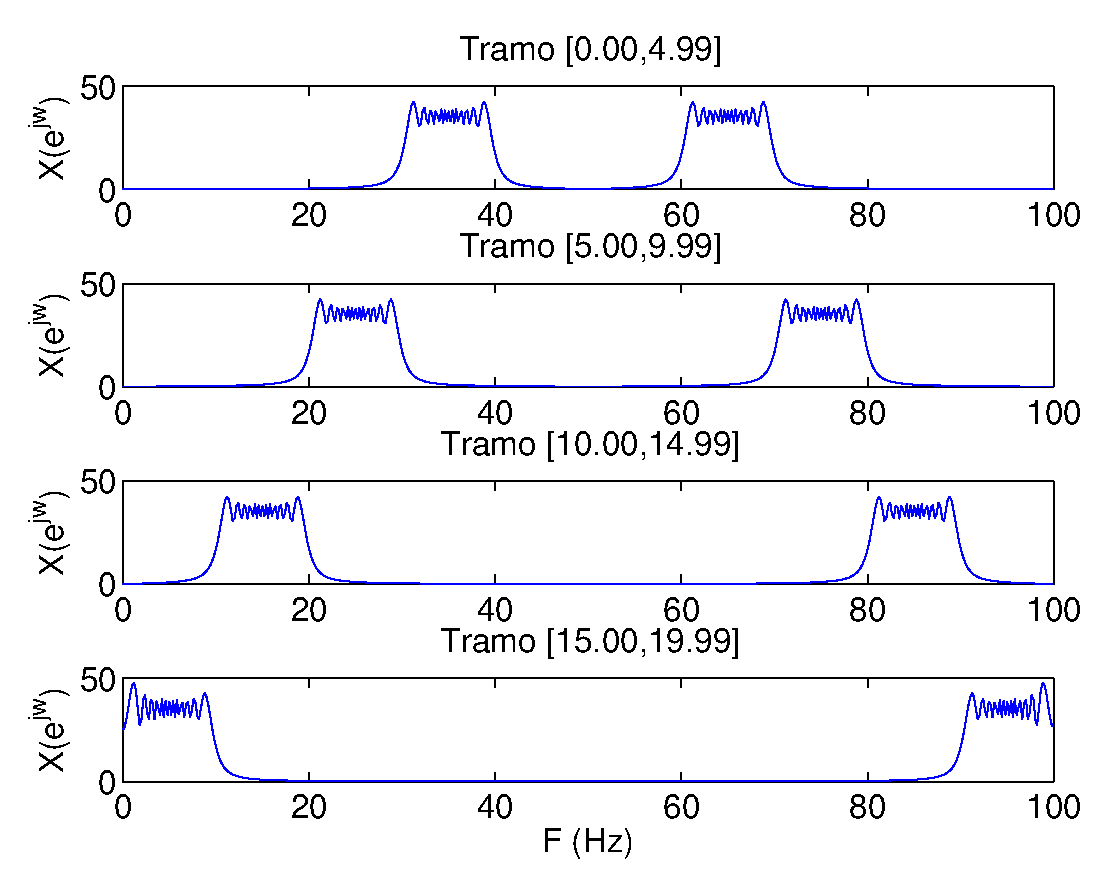
\includegraphics[width=3.5cm]{./Figures/Spect1.eps}


\visible<4->{


\rotatebox{90}{\hspace{0.1cm}\textit{Ventana hamming}}
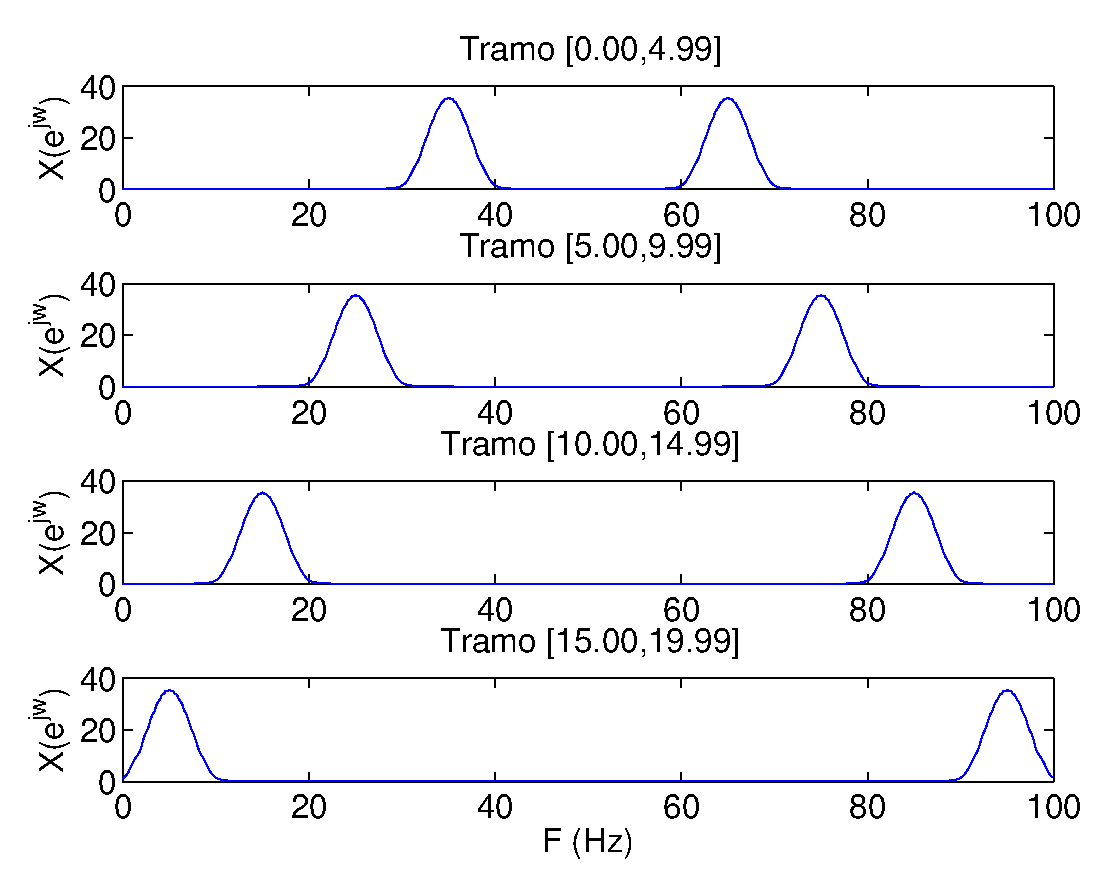
\includegraphics[width=3.5cm]{./Figures/Spect2.eps}
}

\end{column}
\end{columns}
\end{itemize}

\end{frame}

%%%%%%%%%%%%%%%%%%%%%%%%%%%%%%%%%%%%%%%%%


\begin{frame}
\frametitle{Caracterización en frecuencia de señales reales III}

\vspace{-0.2cm}

\footnotesize

\begin{itemize}
\item Adicionalmente, para poder observar con mayor ``resolución temporal'' como cambia el espectro de la señal a lo largo del tiempo, el envenenamiento de la señal se puede realizar sobre tramos sucesivos que se superponen entre si. Es decir, se puede calcular la transformada sobre dos instantes cuya diferencia temporal es más pequeña que el tamaño de la ventana elegida. 

\vspace{-0.4cm}

 \begin{columns}[c]
\begin{column}{6cm}

\visible<3->{

\lstinputlisting{./Matlab/Spect3Corte.m}}

\end{column}

\hspace{-0.8cm}\begin{column}{4cm}

\scriptsize


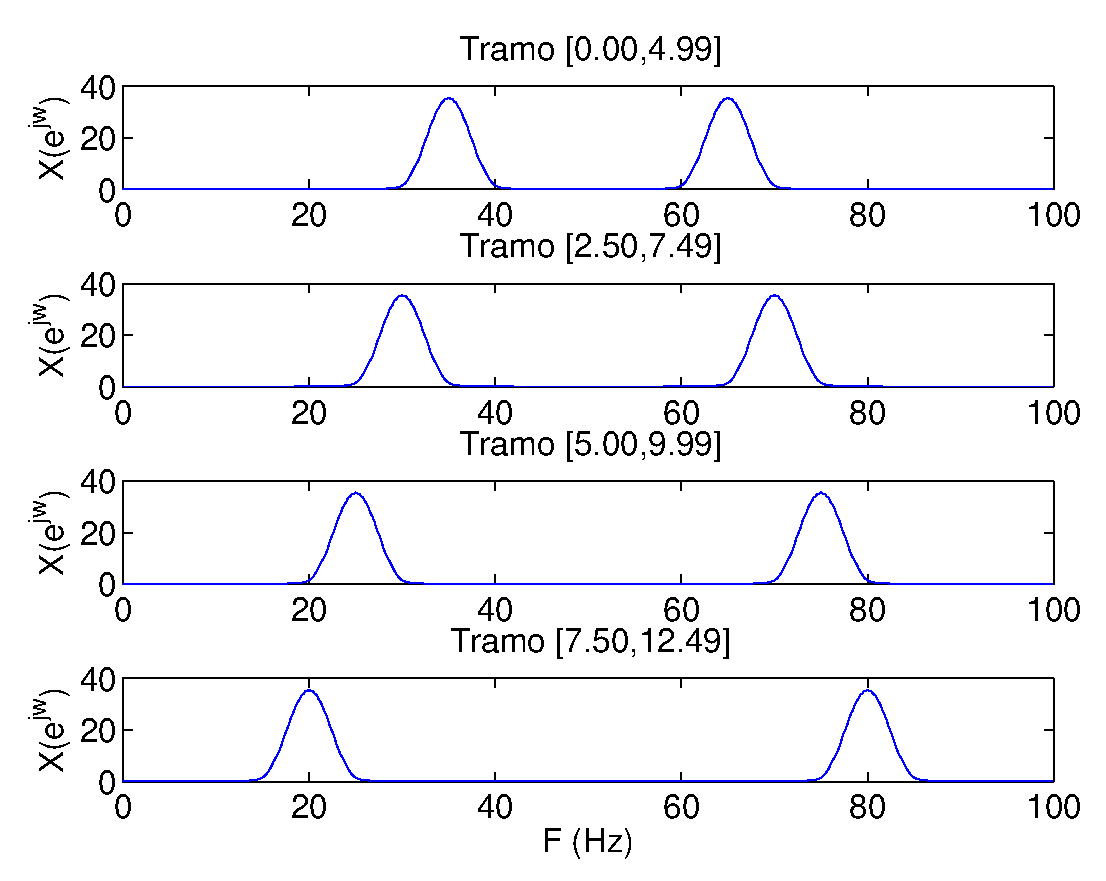
\includegraphics[width=3.5cm]{./Figures/Spect3.eps}


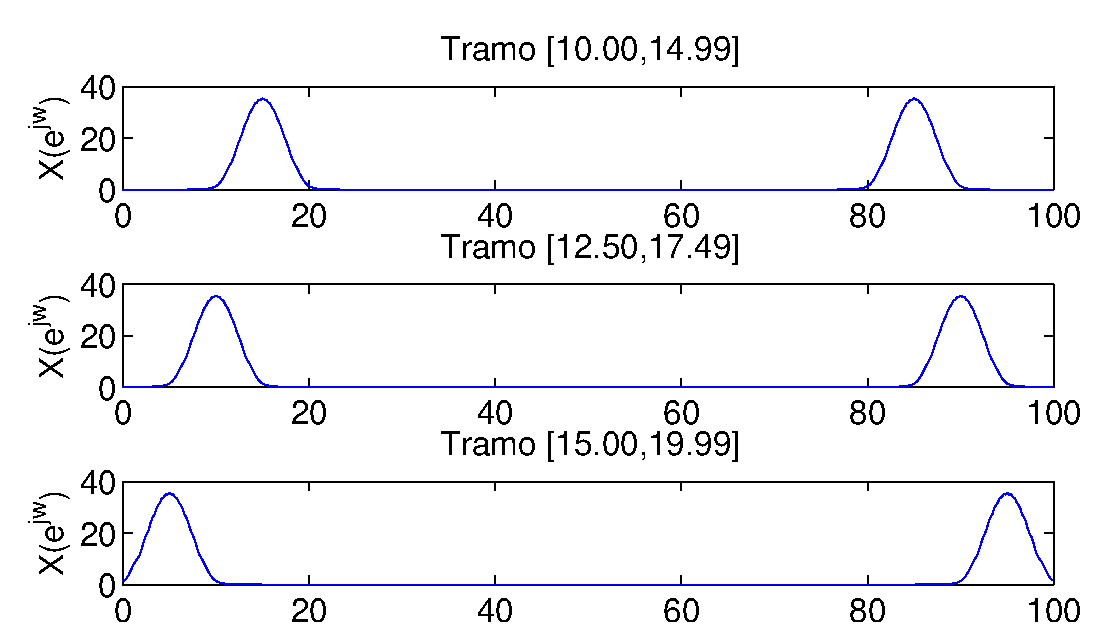
\includegraphics[width=3.5cm]{./Figures/Spect4.eps}

\end{column}
\end{columns}


\end{itemize}

\end{frame}


%%%%%%%%%%%%%%%%%%%%%%%%%%%%%%%%%%%%%%%%%%%%%%%%%

\begin{frame}
\frametitle{Caracterización en frecuencia de señales reales IV}

\vspace{-0.2cm}

\footnotesize

\begin{itemize}

\item Esta forma de proceder, i.e. realizar la Tranformada de Fourier a través de una ventana que se va desplazando a lo largo del tiempo, es lo que se denomina Transformada de Fourier de corta duración (STFT, Short Time Fourier Transform).

\visible<2->{

\item Esta transformada está definida para las transformadas que conocemos: 

\begin{itemize}

\footnotesize


\item Continuo:   $X(jw\visible<3->{,\alert{\tau}})=\int_{-\infty}^{\infty} \visible<3->{\alert{v(t-\tau\visible<4->{,L})}}  x(t) e^{-jwt} dt$

\vspace{0.1cm}

\item Discreto:   $X(e^{jw}\visible<3->{,\alert{n}})=\sum_{k=-\infty}^{\infty} \visible<3->{\alert{v(k-n\visible<4->{,L})}}  x(k) e^{-jwk} $

\vspace{0.2cm}

\visible<5->{

\item Definición análoga para la DFT}

\end{itemize}
}


\visible<3->{

\item El parámetro adicional que aparece en la transformada ($\tau$ o $n$) se encuentra asociado con el desplazamiento de la ventana. Esto implica que exista una transformada diferente para cada instante ($\tau$ o $n$).
}


\visible<4->{

\item El parámetro adicional que aparece en la ventana (L) esta relacionado con su tamaño (2L). Por lo tanto, es el valor que se utiliza para decidir cuantos instantes de tiempo entorno a $\tau$ o $n$ se tienen en cuenta para calcular el espectro en frecuencia.
}

\end{itemize}
\end{frame}

%%%%%%%%%%%%%%%%%%%%%%%%%%%%%%%%%%%%%%%%%%%%%%%%%%%%%%%%%%%%%%%%%%%%%%%%

\begin{frame}
\frametitle{Espectrograma: representación gráfica STFT I}

\vspace{-0.2cm}

\footnotesize

\begin{itemize}

\item Definición de la STFT:

\begin{itemize}

\footnotesize

\item Continuo:   $X(jw,\tau)=\int_{-\infty}^{\infty} v(t-\tau,L)  x(t) e^{-jwt} dt$

\item Discreto:   $X(e^{jw},n)=\sum_{k=-\infty}^{\infty} v(k-n,L)  x(k) e^{-jwk} $

\end{itemize}



\item  Para realizar la representación gráfica de la STFT hay que tener en cuenta de que ésta es una función que depende de dos variables: $w$ y $\tau$/$n$. 

\visible<2->{

\item Por lo tanto, hay que utilizar algún tipo de gráfico en el que se pueda observar como cambian los valores de la STFT según cambia la frecuencia y el tiempo de la señal: 

}

\begin{itemize}
\footnotesize

\visible<3->{

\item La representación que se ha realizado para el caso de la DFT a lo largo de las transparencias, con una gráfica para diferentes regiones de la señal, no es cómoda, ya que requiere de tantas gráficas como instantes $\tau$ o $n$ se quieran muestra.
}

\visible<4->{
\vspace{0.1cm}

\item La alternativa habitual consiste en mostrar los valores de la STFT sobre el plano ($w \times \tau$) o ($w \times n$) utilizando un mapa de colores. 
}

\visible<5->{
\vspace{0.1cm}

\item La orden de Matlab \color{blue}{\texttt{espectrogram}} \color{black} realiza la FFT de corta duración y la representa gráficamente. 
}
\end{itemize}
\end{itemize}

\end{frame}


%%%%%%%%%%%%%%%%%%%%%%%%%%%%%%%%%%%%%%%%%%%%%%%%%%%%%%%%%%%%%%%%%%%%%%%%

\begin{frame}
\frametitle{Espectrograma: representación gráfica STFT II}

\vspace{-0.2cm}

\footnotesize

\begin{itemize}
\item Uso de la orden en Matlab: 

\hspace{1cm} \color{blue}{\texttt{espectrogram(x,window,overlap,[],Fs)}}\color{black}

\vspace{-0.1cm}

\begin{itemize}
\scriptsize
\item \color{blue}\texttt{x}\color{black}: La señal muestreada
\item \color{blue}\texttt{window}\color{black}: El tamaño de una ventana de hamming (valor entero) o la ventana que se quiera utilizar (del tamaño elegido)
\item \color{blue}\texttt{overlap}\color{black}: Entero con los valores que se pueden superponer. Por lo tanto, indirectamente fija el valor del paso de $\tau$ y $n$.
\item \color{blue}\texttt{Fs}\color{black}: Frecuencia de muestreo. Se utiliza para representar correctamente las frecuencias en Hz y el paso temporal de la señal $\tau$ o $n \cdot T_s$.


\vspace{0.3cm}

\visible<2->{
 \begin{columns}[c]
\begin{column}{5cm}



\lstinputlisting{./Matlab/Spect4Corte.m}

\end{column}

\hspace{-0.8cm}\begin{column}{4cm}

\scriptsize


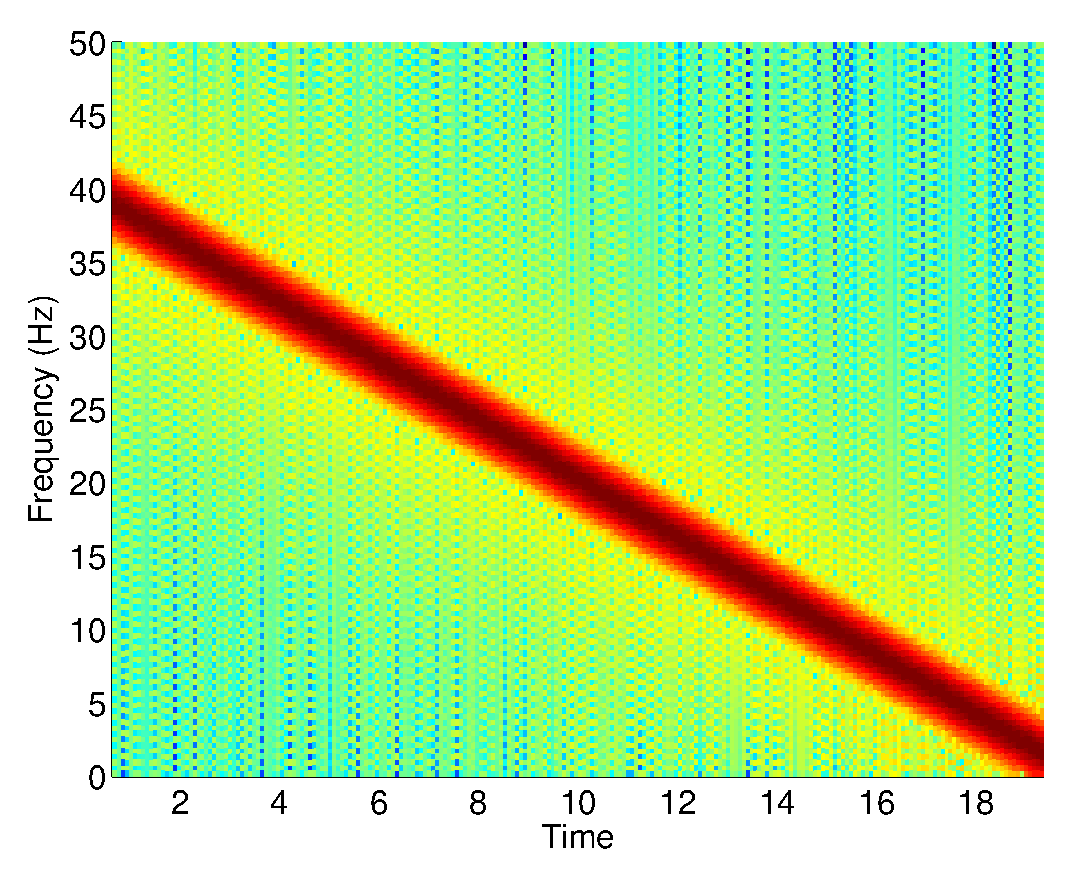
\includegraphics[width=4cm]{./Figures/Spect5.eps}


\end{column}
\end{columns}
}

\end{itemize}

\end{itemize}
\end{frame}






